% Chapter: Server 

This chapter explains overall architecture of the \textan{} sever application. It
provides descriptions of all important components and their interaction.

\section{Server Architecture}

The server architecture is based on a logical multilayered architecture. It
consists of 5 layers: a presentation layer, a service layer, a business logic
layer, a persistence layer and a data layer (see Figure
\ref{fig:ServerComponentOverview}).

\begin{figure}[!htb]
        \centering
        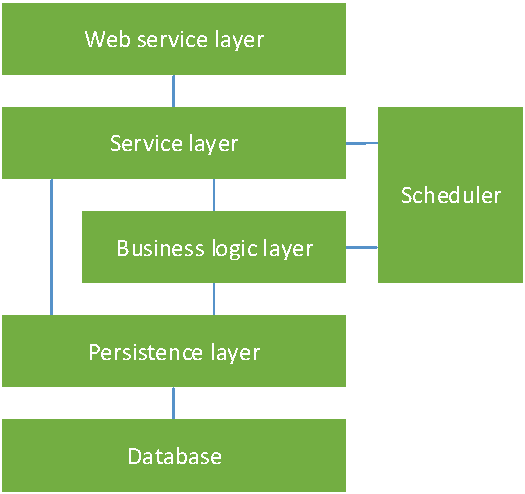
\includegraphics{Images/ServerComponentOverview}
        \caption{Overview of the server layered architecture.}
        \label{fig:ServerComponentOverview}
\end{figure}

\subsection{Web Service Layer}

Web service layer is the component responsible for providing web service
API. It consists of a servlet container and implementations of particular
web services.

Jetty is used as the servlet container component. It is a powerful and scalable
component which supports embedding into other applications.
It also can be run independently on the rest of the application. This is an
important feature, which allows that only web service implementations live in the
web context. In other words, there can be at the same time other components that
access the service layer without usage of the web service layer and still utilize
the full potential of the system. This component also provides security of \textan
server over SSL.

Web service itself is implemented with Apache CXF framework. The bigger part of
the implementation is generated from WSDL files and XML Schema files using the
CXF wsdl2java tool at build time. These classes are placed in the package
\emph{cz.\-cuni.\-mff.\-ufal.\-textan.\-commons.\-ws}, the package
\emph{cz.\-cuni.\-mff.\-ufal.\-textan.\-commons.\-models} and its subpackages.
The *.ws package contains Java equivalents of a WSDL interfaces and the *.models
package contains Java equivalents of XSD complex types. These interfaces are
implemented in classes placed the package \emph{cz.\-cuni.\-mff.\-ufal.\-textan.\-server.\-ws}
and they are just adapters for the service layer. Note that underlaying layers
are totally independent from the web service layer. The CXF framework ensures
that these classes are deployed as servlets.

\subsection{Service Layer}
The service layer is a component that consists of classes which handle requests
using underlying layers and register commands in the scheduler. These classes
are placed in the package \emph{cz.\-cuni.\-mff.\-ufal.\-textan.\-server.\-services}
and the package \emph{cz.\-cuni.\-mff.\-ufal.\-textan.\-server.\-models}.

\comment[Petr]{Petr}{Describe all services}

\subsection{Business Layer}
The business layer contains components which encapsulate the main functionality
of the system. The layer consists of two main components, the Named Entity
recognizer (see \autoref{sec:NamedEntityRecognizer}) and the Object assigner 
(see \autoref{sec:ObjectAssigner}). Both of them use machine learning methods to
solve their tasks. They access the persistence layer to obtain the training
data. They are called from the service layer and the scheduler.

\subsection{Scheduler}
The scheduler is a simple component that invokes commands asynchronously against
requests in the servlet container. It is implemented by classes in the package
\emph{cz.\-cuni.\-mff.\-ufal.\-textan.\-server.\-commands} (see Figure
\ref{fig:CommandsOverview}).

\begin{figure}[!htb]
        \centering
        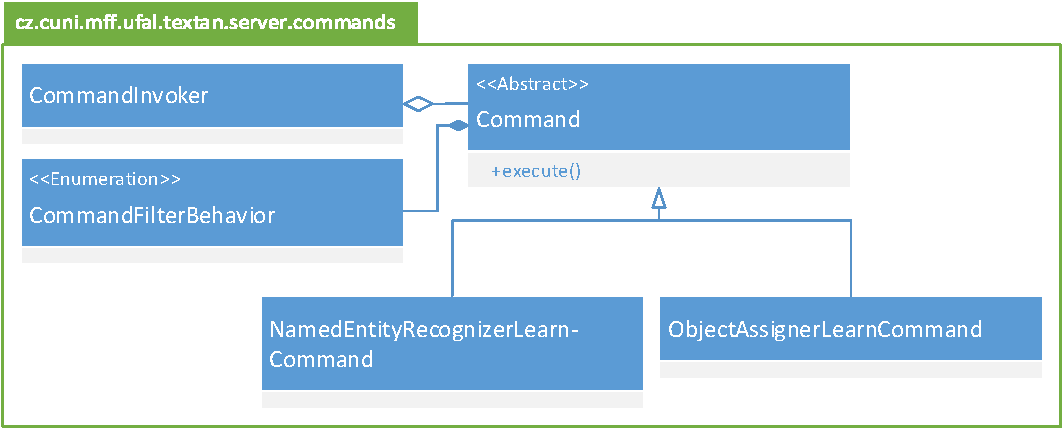
\includegraphics[width=\textwidth]{Images/Commands}
        \caption{Overview of the scheduler classes.}
        \label{fig:CommandsOverview}
\end{figure}

The component is used to invoke re-learning of components from the business
layer. The learning is typically slow, in a matter of minutes, so it's necessary
to use this approach due to system performance. Commands are registered from
methods in the service layer that modify data used for learning. Commands are
stored in one FIFO queue and are invoked in one thread, so it's possible to
filter them before invocation. This ability ensures that only one learning
command is invoked at a time and that learning commands are not invoked
unreasonably. Components from the business layer use old models during learning,
so the re-learning is a transparent operation for users.

\subsection{Persistence Layer}
\label{sec:PersistentLayer}

\comment[Venca]{Petr}{This section is full of bullshit, same as other from you.
Please, use the passive. Also, the main goals of persistence layer (and especially
in dao pattern) is to hide how data are stored and make application independent
from an underlying database. Furthermore, i think that we don't care about transactions,
Spring data cares about transactions and so on.}
\comment[Petr]{Venca}{Feel free to mark bullshits in text}

\comment[Venca]{Petr}{Did you ever write formal text? Or did you ever read any? For example hibernate documentation?}
\comment[Petr]{Venca}{Nope, yep, yep. Thanks for advice.}

Persistence layer takes care about providing data to application layer and
ensure they are persistent. The layer provides conversion of data between database
records and objects in Java. This is called Object-Relation Mapping
(ORM). Java classes whose instances are stored in database tables are called
persistent classes. It is realized via Hibernate ORM framework (see Section
\ref{sec:UsedTechnologies}). Next thing this layer needs to take care of is performing transactions,
for example joining two objects should first check if they are roots and if so, they
are joined. All operations with database are usually done by DAOs.

\begin{figure}[!htb]
        \centering
        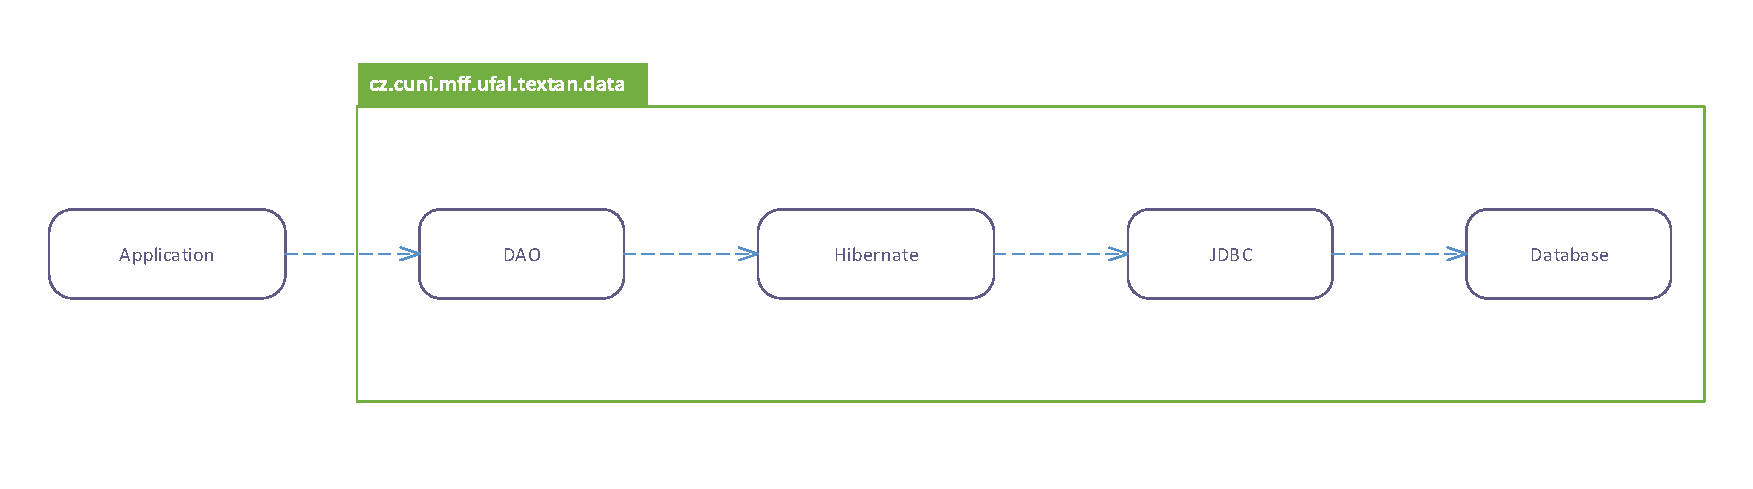
\includegraphics[width=\textwidth]{Images/PersistentLayer}
        \caption{Persistence Layer}
        \label{fig:PersistentLayer}
\end{figure}

Data Access Object (DAO) is a basic design pattern for most of enterprise
applications and wraps all access to data sources. It also handles the
connection to data sources to get and store data. Basically
it is appreciated when the persistence layer changes. For example in case of changing
an underlying database or Hibernate ORM, it is not necessary to remake the whole
application but only the DAO. As you can see in Figure
\ref{fig:PersistentLayer} without DAO would have the application
to call Hibernate functions and it would be dependent on Hibernate. Now the
application does not know anything about Hibernate.

\begin{figure}[!htb]
        \centering
        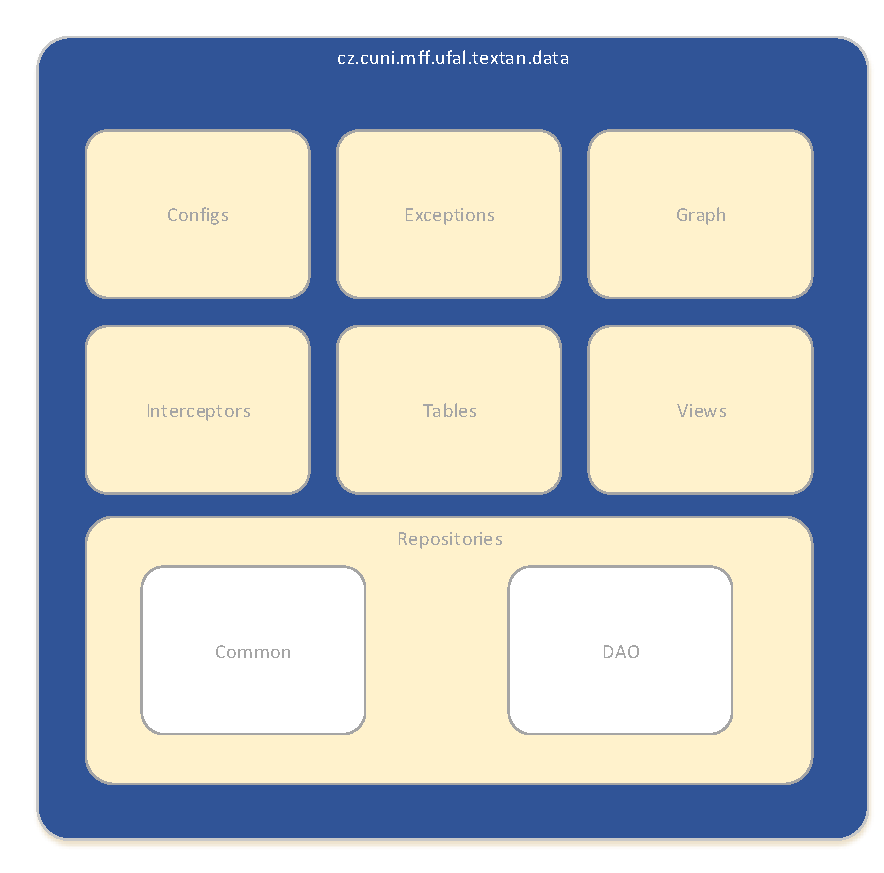
\includegraphics{Images/DataDecomposition}
        \caption{Persistence Layer Decomposition}
        \label{fig:DataDecomposition}
\end{figure}

Figure \ref{fig:DataDecomposition} describes that our persistence layer is
covered by package \emph{cz.\-cuni.\-mff.\-ufal.\-textan.\-data}. In this section when it is
mentioned some subpackage, it always mean the subpackage of the package \emph{data}.

The mapping between tables in the database and Java classes is done in
subpackage \emph{tables}. Every table in the database corresponds to a class
that extends \emph{AbstractTable}. Hibernate does the mapping for us.

\begin{figure}[!htb]
        \centering
        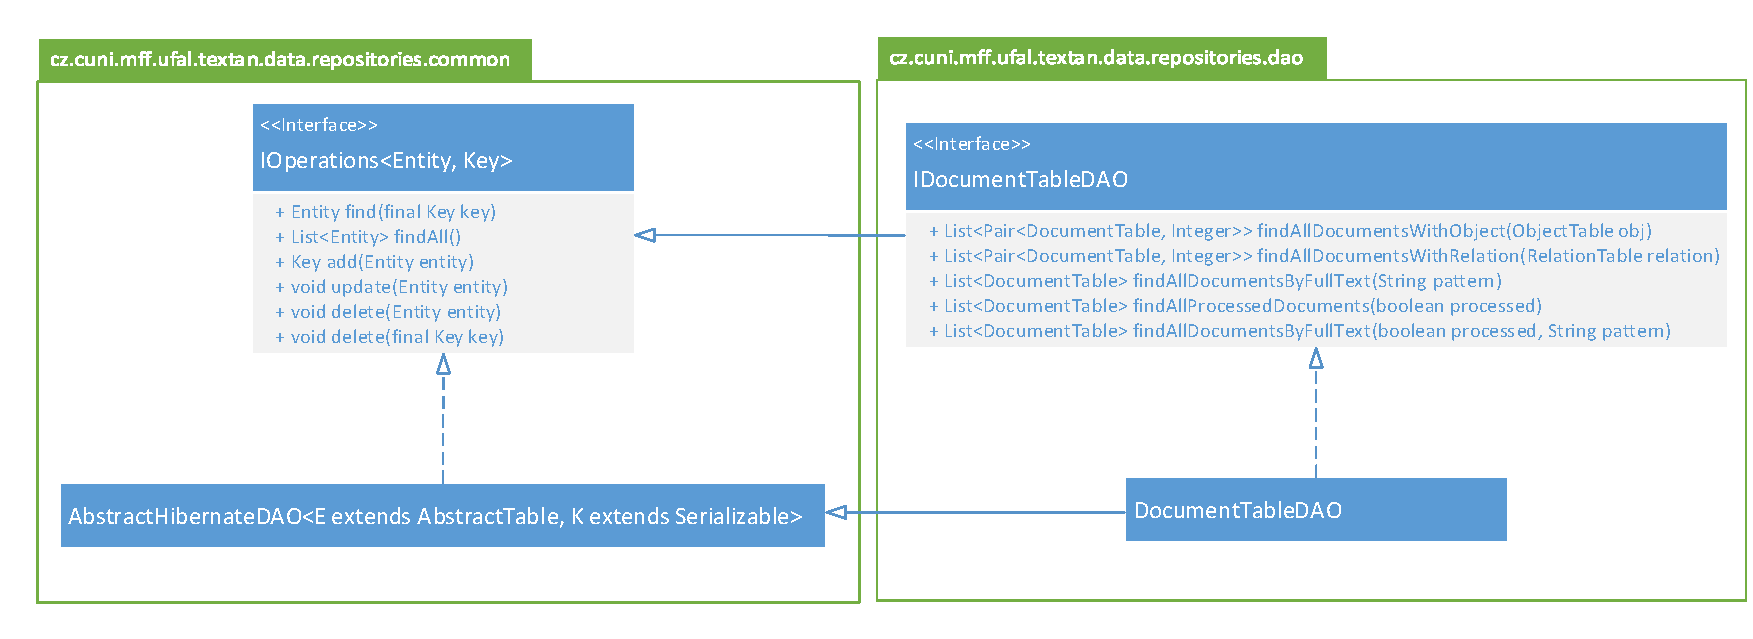
\includegraphics[width=\textwidth]{Images/DatabaseDAO}
        \caption{DAO Example for Document Table}
        \label{fig:DatabaseDAO}
\end{figure}

The DAO pattern is used to provide the data to upper layers as it is mentioned
earlier. DAOs are located in subpackage \emph{repositories}.
In Figure \ref{fig:DatabaseDAO} there is an example of a
DAO pattern for document table. Interface \emph{IOperations} describes common
methods for all tables and \emph{AbstractHibernateDAO} implements them. For
example for the document table we have interface \emph{IDocumentTableDAO} that
describes all operations with document table and \emph{DocumentTableDAO}
implements them using Hibernate. The application (server) itself should not know
about the implementations to guarantee the independence on Hibernate.

Another subpackage \emph{graph} contains all necessary methods to generate a
graph from database. Nodes of this graph represents objects and relations in
the database. Edge between an object and a relation means that this object is in
that relation. It is used the factory pattern to create the graph. There are
methods in class \emph{GraphFactory} to generate a graph from an object to given
depth and also methods supporting finding shortest path between two objects.	
There are many algorithms for this purpose. We have
used a simplified \emph{Bidirectional search} because we want to use as least memory as
possible and it can take twice less memory than standard BFS.

The last interesting subpackage is \emph{interceptors} containing definitions
of Hibernate interceptors. Interceptor is something like trigger in a database.
When insert, update or delete action are called in hibernate, a proper method
in an interceptor is called. It is used for \emph{global version} which we
discuss in Section \ref{sec:Database}.

A part of the persistence layer is also a full text indexing and searching. It is
done through Hibernate Search framework (see Section \ref{sec:UsedTechnologies}),
which makes the server application more independent from an underlying database.
The indexing is done in two places in the server application: at start up and at
database change using Hibernate ORM. A disadvantage of this approach is that
an underlying database must be changed only through one instance of the server
application, otherwise full text indexes become inconsistent with data in the database.
An integration of the framework into the layer is done using mappings for persistent
objects and special queries in DAO.

\subsection{Database}
\label{sec:Database}

This section describes the database schema (see Figure \ref{fig:DatabaseSchema}),
meaning of all database tables and columns.

\begin{figure}[!hp]
        \centering
        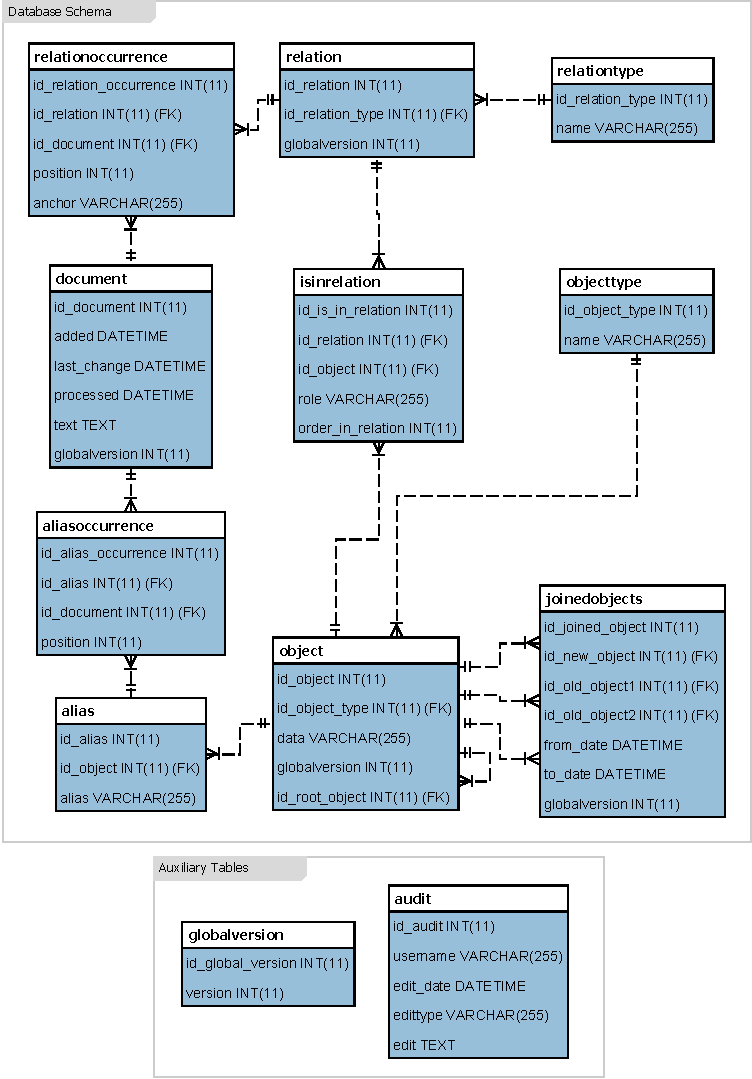
\includegraphics{Images/DatabaseSchema}
        \caption{Database schema}
        \label{fig:DatabaseSchema}
\end{figure}

\paragraph{Document} The report to be processed. In the database, there are
columns for the date of creation (\emph{added}), the date for last change and
the date when the document has been processed.

\paragraph{Object} Records in this table represent objects, e.g. concrete person
called Josef Novák or a specific address.  It contains reference to
\emph{ObjectType} table to determine what type the object is.

\paragraph{Object Type} The \emph{objecttype} table is used to describe if the
object is a human or an address. It has only one meaningful column with name of
the type and the types have to be unique.

\paragraph{Alias} If an entity occurs in some document, we want to know what it
was called. For instance Josef Omáčka can be called as ``Josef'', ``Pepe'' or
``Killer''. Alias table represents all these possibilities (aliases) 
of a specific object.

\paragraph{Relation} There may be relations between objects, for example
killer-victim, mother-son, live, use, etc. This table describes such
relationships. 

\paragraph{IsInRelation} There can be relation between more than two entities,
for example  killer-victim-place-time. This is the reason we have used the N:N
relation  between \emph{object} and \emph{relation} tables which represents the
\emph{isinrelation} table. For instance, to distinguish between killer and
victim, the column \emph{role} has been used.

\paragraph{RelationType} As well as the objects have types, the relations have their
types too. For example ``kill'', ``live'' or ``sell''.

\paragraph{Relation and Alias Occurrences} These two tables stand for the
occurrence of an alias or relation in a document respectively. It contains their
beginning positions in the document and an anchor for relation. 

\paragraph{Joined Objects} It is possible that users may realize two different
objects are actually a single one. In this case, two objects have to be joined
into a new one. This can be done by \emph{joinedobjects} table. However, this
join can be a wrong decision. There is a column to\_{}date in case these merged
objects are separated.

\paragraph{Audit} All inserts, deletes and updates in the tables above are being
saved into \emph{audit} table. It is a simple table because it keeps a string of
modified object. It also keeps the username of the user who performed the
operation, the date of the change and what kind of change was performed.
 
\paragraph{Global Version} Before finishing the processing of a document, it is
checked whether there are other documents which have been added or modified
during the processing. To perform that check we need to have some information
when the tables have been modified. Tables \emph{Document}, \emph{Object} and
\emph{Relation} contain a column \emph{globalversion}, which increments with
each insert, delete or update. Current global version is stored in
\emph{globalversion} table where there is only a single row every time.

\paragraph{} There is a little bit of redundancy in our schema.
There is alias table where the alias of an object is stored. But if we really
want to extract the alias of an object, we could get the alias from document,
which the object occurs. However, that would be too complicated to get from
single query. Furthermore, we want a method to easily get all aliases of an
object.

Next redundancy is \emph{Object.id\_{}root\_{}object} which is a foreign key of
the same table. Joining two objects into a new one repeatedly
makes a binary tree. A root of the tree is the object whose aliases are being
edited, because other objects in the tree are not taken into account. So there are needed two operations: to determine if a given object is a root and to get the
root of an object. Without column \emph{Object.id\_{}root\_{}object} we would have to
join until we get to the root and that, as we know, cannot be done in a single
SQL query. With the column \emph{Object.id\_{}root\_{}object}, we only ask whether the \emph{Object.id\_{}root\_{}object} is equal to \emph{Object.id} or we simply get the root object in one join.

There was a discussion about the equivalence between object and relation. It
seems both sides (relation type, relation, relation occurrence versus object type,
object, alias, alias occurrence) look pretty much the same. Someone had an
opinion that relation is just an object. But there are several reason why we
have a separate table for relations. Relations cannot be joined like objects, we
do not care too much about the alias and there could be problem in the 
\emph{IsInRelation} table where two objects could be assigned instead of an
object and a relation. Relations are just way too different from objects, so we
decided to give them extra table.

\section{Named Entity Recognizer}
\label{sec:NamedEntityRecognizer}

The architecture of Named entity recognizer is divided to two parts: recognition
and training.

\paragraph{Recognition} 
Recognition is split into two parts - Java part and C++ part. This is because
NameTag, which is the available tool for named entity recognizer, is written
mainly in C++. \textan{} is developed in Java, so we must use JNI to call
functions from C++ through provided Java bindings. C++ part is represented by
NameTag, so it has its own documentation. Java part contains JNI bindings to
call C++ part and the connection to \textan{}. This part serves as an adaptor
between these two projects. Its main task is to translate recognized NameTag
entities to entities stored in \textan{} database. Because of optimization, this
component caches database entities.

\paragraph{Training}
Despite the fact that NameTag is in C++ and \textan{} in Java, it is not
requisite to implement JNI, because training is called as binary files and the
model is generated as file. Therefore, calling C++ functions is not needed. Java
part provides training data collecting from database and preparation, model
handling (deleting old ones and binding them to NameTag).
\comment[Jakub, Petr]{Tam}{Approved?}

\subsection{Methods}
This part explains methods used in NameTag. \comment[]{Jakub}{add source - Fox paper http://ufal.mff.cuni.cz/~straka/papers/2013-tsd\_ner.pdf}

\subsubsection{System overview}
NameTag is based on Maximum Entropy Markov Model (MEMM). Its output is used for a Viterby decoder, which decodes probabilities estimated by a MEMM classifier.
At the beginning, for each word the full probability distribution of its classes and positions with respect to an entity is predicted by maximum entropy model. Than, output is optimized via dynamic programming, which determines the optimal combination of classes and named entity chunks.
Whole pipeline runs two times, using the output of first iteration as an additional feature for second iteration.

\subsubsection{Maximum Entropy Classifier}
First task of classifier is to predict for each word the named entity type and position in the entity. Positions are described with a {\it BILOU} model (B-beginning of multiword entity, I-inside word of multiword entity, L-last word of multiword entity, O-outside any entity, U-unit word entity).

\subsection{Decoding}
The probabilities estimated by the maximum entropy model are decoded with the Viterbi algorithm implementation. Than, optimization is used-impossible combinations of {\it BILOU} positions are discarded, which leads (in combination with dynamic programing) to complexity  \(O(N \cdot C)\), where \(N\) is the number of words in a sentence.

\subsubsection{Classification Features}
Maximum entropy classifier uses this features: form, lemma, tag, chunk (English only) of current word and surrounding words in window
\pm 2, orthographic features (capitalization, punctuation, lowercase and uppercase form of
the word), suffixes and prefixes of length 4 and regular expressions identifying possible
year, date and time (Czech only).
Besides features based on word and its neighbors, global features are used too. In second pipeline stage, information about prediction of five adjacent word is used (both directions) and information about the previous prediction of the candidate word in 500 preceding words.

\section{Object Assigner}
\label{sec:ObjectAssigner}

After calling \emph{Named entity recognizer}, a list of entities is extracted
from the document. \emph{ObjectAssigner} package \emph{cz.\-cuni.\-mff.\-ufal.\-textan.\-assigner}
automatically assigns those entities to
available objects in the database. As the output, for each entity, the
aforementioned package returns a list of potential objects along
with their score. Figure~\ref{fig:objectassigner} illustrates 
how the object assigner is organized. As can be seen, the package offers 
two methods assigning objects to the entity.

\begin{figure}[!htb]
        \centering
        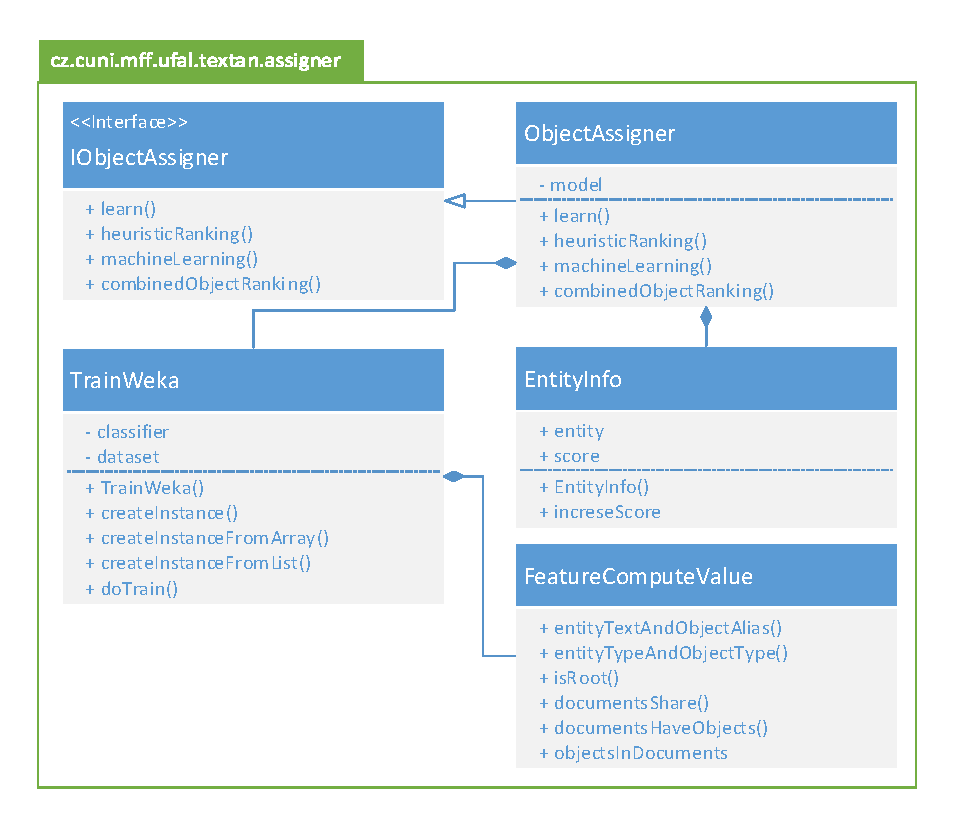
\includegraphics[width=\textwidth]{Images/ObjectAssignerClass}
        \caption{Object Assigner Class Diagram}
        \label{fig:objectassigner}
\end{figure}


\paragraph{HeuristicRank}
The simplest solution is searching for the \textit{objects} with matching 
\textit{alias}. However, for an array of entity, it would return an array of 
list of unordered objects. Function
\emph{cz.\-cuni.\-mff.\-ufal.\-textan.\-assigner.\-ObjectAssigner.\-HeuristicRanking}
loops through the whole structure, promote the pair of objects which has a
relation. This is due to the fact that such pair of objects is more likely to
appear in the same document. However, as a heuristic method, its main role is to
guarantee a decent output for every input.

\paragraph{MachineLearning}
Without extensive human effort, machine learning is the best method to achieve
high performance from a huge database. The problem of ``matching potential
objects to an entity'' is reformulated to fit the definition of a classification
machine learning. Each object is paired with the entity. Then the pair is
classified as \emph{positive} if the object is potentially matched the entity.
Otherwise, the pair is classified as \emph{negative}. It becomes the
problem of binary classification.


\paragraph{Learning}
The package \emph{cz.\-cuni.\-mff.\-ufal.\-textan.\-assigner.\-data} supports all steps for
machine learning including training (learning). The database is extracted. 
\emph{cz.\-cuni.\-mff.\-ufal.\-textan.\-assigner.\-data} creates artificial pairs of
training vectors with \textit{Weka} tool. When a new document is processed,
new entity and object pairs are added to the database. They could be extracted
later to train again.

\paragraph{Assigning}
To assign the entity to object, function \emph{distributionForInstance} returns
the probability of the pair with regards to \emph{positive} class. The
probability value is ranked and used as the score.

\paragraph{Features}

The feature set is selected among evaluations with regards to the pair between
the entity and the object. A feature could be computed by comparing the entity 
and the object. It also may be the characteristics of the entity or the object 
alone. All the features are considered to create a meaningful set which
expresses the nature of the pair. The final feature set is selected 
as follow:

\begin{itemize}
\item The String distance metrics between the entity text and the object
aliases. Given the fact that an object may have more than one alias, the package
computes three numbers for \textit{similarity} between the entity text and the
object aliases: the highest, the lowest and the average. It is to distinguish
between an object with one alias and object with hundred aliases.
\item The type comparison between object type and entity type. If a pair is
\textit{positive}, the types have to be the same. This is a crucial feature. 
\item A check if the object is the root. It is a fact that the root of
\textit{joined} object should have higher priority than non-root object.
\item The number of neighbors that the object has. This feature takes into
consideration the number of relations that the object has.
\item The number of Document occurrences that the object appears.
\item The number of Document occurrences that the entity appears.
\item The number of documents where the object and the entity appear together.
\item The number of documents that the entity and neighbors of the object appear together.
\item The number of neighbors of the objects that happen to be in the same document with the entity.
\end{itemize}


